\documentclass[11pt]{article}
\usepackage{amsmath,amssymb,amsthm}
\usepackage{graphics}
\usepackage{graphicx}
\usepackage{float}
\usepackage[margin=1in]{geometry}
\usepackage{algorithm}
\usepackage{algpseudocode}
%\usepackage{hyperref}
\usepackage{subfigure}

% Macros
\newcommand{\KK}{\mathcal{K}_k}
\newcommand{\Ik}{\begin{pmatrix} I_{k-1} \\ 0\end{pmatrix}}
\newcommand{\hQ}{\hat{Q}}


\begin{document}
\title{CME338 Final Project\\
LSLQ Solver }
\author{Ron Estrin and Anjan Dwaraknath}
\date{}
\maketitle

\section{Introduction}
In the spirit of LSQR and LSMR, which apply CG and MINRES respectively to the normal equations, we derive LSLQ, which applies SYMMLQ to the normal equations. Starting from the normal equations, and SYMMLQ subproblem, we derive short recurrences for the computation of iterates and residual norm estimates. We then evaluate the effectiveness of SYMMLQ on some linear systems and least-squares problems, and make comparisons to LSMR.

\subsection{Notation}
We denote matrices by capital letters, vectors by lower case letters, and scalars are denoted by greek lower case letters. There will be some occasions where we abuse matrix notation by multiplying matrices of incorrect sizes when the matrices are meant to be applied to only a subset of the rows or columns of another matrix.
We denote the Krylov subspace of size $k$ by 
$$\KK = \KK (A^T A, b) = \mathrm{span}\left(b, A^T A b, \dots, (A^T A)^{k-1} b \right)$$.

\section{Derivation of LSLQ}
In this section, we derive the short recurrence formulas for LSLQ beginning from the Golub-Kahan process.

\subsection{Golub-Kahan Process}
The Golub-Kahan process is defined by the recurrence defined in Algorithm \ref{GK}.

\begin{algorithm}
\caption{Golub-Kahan Process}
\label{GK}
\begin{algorithmic}
	\State Set $\beta_1 u_1 = b$, $\alpha_1 v_1 = A^T u_1$
	\For{$k=1,2,\dots$}
		\State $\beta_{k+1} u_{k+1} = A v_k - \alpha_k u_k$
		\State $\alpha_{k+1} v_{k+1} = A^T u_{k+1} - \beta_{k+1} v_k$
	\EndFor
\end{algorithmic}
\end{algorithm}

After performing $k$ iterations of this process, we obtain the decompositions

\begin{eqnarray}
\label{GKdcmp1}
A V_k &=& U_{k+1} B_k \\
\label{GKdcmp2}
A^T U_{k+1} &=& V_{k+1} L^T_{k+1}.
\end{eqnarray}

where $U_k = \left( u_1  | \dots | u_k \right)$, $V_k = \left( v_1 | \dots | v_k \right)$, and

\begin{equation*}
B_k = \begin{pmatrix}
\alpha_1 & & & \\
\beta_2 & \alpha_2 & & \\
 & \ddots & \ddots & \\
 & & \beta_k & \alpha_k \\
 & & & \beta_{k+1} 
\end{pmatrix} \qquad L_{k+1} = \begin{pmatrix}
B_{k+1} | \alpha_{k+1} e_{k+1}
\end{pmatrix}.
\end{equation*}

We can then observe that $V_k$ is a basis for $\KK (A^T A, b)$, since

$$ A^T A V_k = A^T U_{k+1} B_k = V_{k+1} L^T_{k+1} B_k = V_{k+1} \begin{pmatrix}
B^T_k B_k \\
\alpha_{k+1} \beta_{k+1} e^T_k
\end{pmatrix}.
$$

\subsection{The LSLQ subproblem}
In order to solve the linear system or least squares problem $Ax = b$, we instead solve the normal equations $A^T A = A^T b$. Since $A^T A$ is symmetric positive semidefinite and we assume that the normal equations are consistent, we may consider applying SYMMLQ to this system.
We solve the normal equations iteratively, where at iteration $k$ we solve the problem

\begin{equation}
\label{lslqsubproblem}
\begin{aligned}
x_k =&& \underset{x \in \KK}{\arg\min} && \Vert x \Vert_2 \\
&& \text{s.t.} && A^T r \perp \mathcal{K}_{k-1}.
\end{aligned}
\end{equation}

where $r = b - Ax$.

In order to solve this problem, we first note that we may formulate this as an unconstrained problem in a smaller space if we minimize in $y_k$ and set $x_k = V_k y_k$. Then

\begin{eqnarray*}
0 = V_{k-1}^T A^T r_k &=& V_{k-1}^T A^T (b - Ax_k) \\
&=& V_{k-1}^T A^T b - V_{k-1}^T A^T A V_k y_k \\
&=& \alpha_1 \beta_1 e_1 - B_{k-1}^T U_k^T A V_k y_k \\
&=& \alpha_1 \beta_1 e_1 - B_{k-1}^T L_k y_k.
\end{eqnarray*}

Thus in order to solve \ref{lslqsubproblem}, we can solve

\begin{equation}
\label{lslqsubproblemy}
\begin{aligned}
y_k =&& \underset{y \in \mathbb{R}^k}{\arg\min} && \Vert y \Vert_2 \\
&& \text{s.t.} && B_{k-1}^T L_k y = \alpha_1 \beta_1 e_1.
\end{aligned}
\end{equation}

\subsection{First QR decomposition}
We first take the QR factorization of $Q_k R_k = B_{k-1}$. Suppose we have the QR factorization of $Q_{k-1}R_{k-1} = B_{k-2}$, with

\begin{equation*}
R_{k-1} = \begin{pmatrix}
\rho_1 & \theta_2 & & \\
& \rho_2 & \ddots & \\
& & \ddots & \theta_{k-1} \\
& & & \rho_{k-2}
\end{pmatrix}.
\end{equation*}

Then we may recurse to obtain the factorization of $B_{k-1}$

\begin{eqnarray*}
B_{k-1} &=&
\begin{pmatrix}\begin{array}{c|c}
\begin{matrix}
  \alpha_1  &          &         &      \\
  \beta_2   & \alpha_2 &         &      \\
            & \ddots   & \ddots  &      \\
            &          & \beta_{k-2} & \alpha_{k-2} \\
		        &          &         & \beta_{k-1}
 \end{matrix}
&  \begin{matrix} 0 \\ \vdots \\ \vdots \\ 0 \\ \alpha_{k-1} \end{matrix} \\
\hline
\begin{matrix} 0 & \cdots  & \cdots & 0  \end{matrix} & \beta_{k}
\end{array}\end{pmatrix}
 = Q_{k-1}
\begin{pmatrix}\begin{array}{c|c}
\begin{matrix}
 \rho_1     & \theta_2 &         &      \\
            & \rho_2   & \ddots  &      \\
            &          & \ddots  & \theta_{k-2}     \\
            &          &         & \rho_{k-2} \\
		    &          &         & 0 
 \end{matrix}
&  \begin{matrix} 0 \\ \vdots \\ 0 \\ \theta_{k-1} \\ \hat{\rho}_{k-1} \end{matrix} \\
\hline
\begin{matrix} 0 & \cdots  & \cdots & 0  \end{matrix} & \beta_{k}
\end{array}\end{pmatrix} \\
&=& Q_{k-1} G^{(1)}_k
\begin{pmatrix}\begin{array}{c|c}
\begin{matrix}
 \rho_1    & \theta_2 &         &      \\
            & \rho_2   & \ddots  &      \\
            &          & \ddots  & \theta_{k-2}     \\
            &          &         & \rho_{k-2} \\
		        &          &         & 0 
 \end{matrix}
&  \begin{matrix} 0 \\ \vdots \\ \vdots \\ \theta_{k-1} \\ \rho_{k-1} \end{matrix} \\
\hline
\begin{matrix} 0 & \cdots  & \cdots & 0  \end{matrix} & 0
\end{array}\end{pmatrix} = Q_{k-1} G^{(1)}_k
\begin{pmatrix}
R_{k-1} \\
\hline
0 \end{pmatrix},
\end{eqnarray*}
by defining $Q_k = Q_{k-1}G^{(1)}_k$, where $G^{(1)}_k$ is the Givens rotation
$$G^{(1)}_k = \begin{pmatrix}
c_1 & s_1 \\
-s_1 & c_1
\end{pmatrix}. $$
Note that we are abusing notation, where we intend $G_k^{(1)}$ to be applied to rows $k-2$ and $k-1$. 
Using $G^{(2)}_{k-1}$ defined in the previous iteration, we have
\[ \begin{pmatrix} \theta_{k-1} \\ \hat{\rho}_{k-1} \end{pmatrix}
= \begin{pmatrix}  
c^{(k-1)}_1 & -s^{(k-1)}_1 \\
s^{(k-1)}_1 & c^{(k-1)}_1 \end{pmatrix}
\begin{pmatrix} 0 \\ \alpha_{k-1} \end{pmatrix},
\]
\[
\begin{pmatrix} \theta_{k} \\ \hat{\rho}_{k} \end{pmatrix}
= \begin{pmatrix}  c_1 & -s_1 \\ s_1 & c_1 \end{pmatrix}
\begin{pmatrix} 0 \\ \alpha_{k} \end{pmatrix},
\]
\[ \begin{pmatrix} \rho_{k-1} \\ 0 \end{pmatrix}
= \begin{pmatrix}  c_1 & -s_1 \\ s_1 & c_1 \end{pmatrix}
\begin{pmatrix} \hat{\rho}_{k-1} \\ \beta_k \end{pmatrix},
\]
and we therefore obtain the recurrences
\begin{eqnarray}
\hat{\rho}_{k-1} &=& \frac{\alpha_{k-1}\hat{\rho}_{k-2}}{\rho_{k-2}} = c_1^{(k-1)}\alpha_{k-1}, \\
\rho_{k-1} &=& \sqrt{\hat{\rho}^2_{k-1} + \beta^2_k }, \\
c_1 &=& \hat{\rho}_{k-1}/\rho_{k-1}, \\
s_1 &=& -\beta_k/\rho_{k-1}, \\
\theta_{k} &=& \frac{\alpha_k\beta_k}{\rho_{k-1}} = -s_1 \alpha_k.
\end{eqnarray}

\subsection{Forward Substitution}
With the previous QR decomposition, the system we intend to solve becomes
\begin{eqnarray*} 
\begin{pmatrix}
\alpha_1\beta_1 \\ 0 \\ \vdots \\ 0
\end{pmatrix} &=& \begin{pmatrix}\begin{array}{c|c}
 B^T_{k-1}B_{k-1} &  \begin{matrix} 0 \\ \vdots \\ 0  \\ \alpha_k\beta_k \end{matrix} 
\end{array}\end{pmatrix} y_k 
= \begin{pmatrix}\begin{array}{c|c}
 R^T_{k}R_{k} &  \begin{matrix} 0 \\ \vdots \\ 0  \\ \alpha_k\beta_k \end{matrix} 
\end{array}\end{pmatrix} y_k \\
&=& R^T_{k} \begin{pmatrix}\begin{array}{c|c}
 R_{k} &  \begin{matrix} 0 \\ \vdots \\ 0  \\ \frac{\alpha_k\beta_k}{\rho_{k-1}} \end{matrix} 
\end{array}\end{pmatrix} y_k
= R^T_{k} \begin{pmatrix}\begin{array}{c|c}
 R_{k} &  \begin{matrix} 0 \\ \vdots \\ 0  \\ \theta_{k} \end{matrix} 
\end{array}\end{pmatrix} y_k.
\end{eqnarray*}

Define
\begin{equation}
z_k = \begin{pmatrix}
\zeta_2 \\ \vdots \\ \zeta_{k}
\end{pmatrix} = \begin{pmatrix}\begin{array}{c|c}
 R_{k} &  \begin{matrix} 0 \\ \vdots \\ 0  \\ \theta_{k} \end{matrix} 
\end{array}\end{pmatrix} y_k = \tilde{R}_k y_k
\end{equation}
so that we have $R^T_k z_k = \alpha_1 \beta_1 e_1$.
As in the Conjugate Gradient method, we obtain a short recurrence for $\zeta_k$,
\begin{equation}
\zeta_k = -\frac{\theta_{k-1}}{\rho_{k-1}} \zeta_{k-1}.
\end{equation}

\subsection{Second QR decomposition}
Using the recurrence of the previous section, we now need to solve the minimum norm problem
$$ \tilde{R}_k y_k = z_k. $$
We accomplish this by taking the QR decomposition of $\hat{Q_k}\hat{R_k} = \tilde{R}^T_k$. Suppose we have the QR decomposition from the previous iteration, $\hQ_{k-1}\hat{R}_{k-1} = \tilde{R}^T_{k-1}$, with

\begin{equation*}
\hat{R}_{k-1} = \begin{pmatrix}
\sigma_1 & \eta_2 & & \\
& \sigma_2 & \ddots & \\
& & \ddots & \eta_{k-1} \\
& & & \sigma_{k-2}
\end{pmatrix}.
\end{equation*}

Then as was done in the first QR decomposition, we can recurse to obtain a fast update for the second QR decomposition.

\begin{eqnarray*}
\tilde{R}_k^T &=&
\begin{pmatrix}\begin{array}{c|c}
\begin{matrix}
  \rho_1  &          &         &      \\
  \theta_2   & \rho_2 &         &      \\
            & \ddots   & \ddots  &      \\
            &          & \theta_{k-2} & \rho_{k-2} \\
		        &          &         & \theta_{k-1}
 \end{matrix}
&  \begin{matrix} 0 \\ \vdots \\ \vdots \\ 0 \\ \rho_{k-1} \end{matrix} \\
\hline
\begin{matrix} 0 & \cdots  & \cdots & 0  \end{matrix} & \theta_{k}
\end{array}\end{pmatrix}
= \hQ_k
\begin{pmatrix}\begin{array}{c|c}
\begin{matrix}
 \sigma_1    & \eta_2 &         &      \\
            & \sigma_2   & \ddots  &      \\
            &          & \ddots  & \eta_{k-2}     \\
            &          &         & \sigma_{k-2} \\
		        &          &         & 0 
 \end{matrix}
&  \begin{matrix} 0 \\ \vdots \\ \vdots \\ \eta_{k-1} \\ \hat{\sigma}_{k-1} \end{matrix} \\
\hline
\begin{matrix} 0 & \cdots  & \cdots & 0  \end{matrix} & \theta_{k}
\end{array}\end{pmatrix} \\
 &=& \hQ_k G^{(2)}_k
\begin{pmatrix}\begin{array}{c|c}
\begin{matrix}
 \sigma_1    & \eta_2 &         &      \\
            & \sigma_2   & \ddots  &      \\
            &          & \ddots  & \eta_{k-2}     \\
            &          &         & \sigma_{k-2} \\
		        &          &         & 0 
 \end{matrix}
&  \begin{matrix} 0 \\ \vdots \\ \vdots \\ \eta_{k-1} \\ \sigma_{k-1} \end{matrix} \\
\hline
\begin{matrix} 0 & \cdots  & \cdots & 0  \end{matrix} & 0
\end{array}\end{pmatrix}
\end{eqnarray*}

We define $\hQ_k = \hQ_{k-1}G^{(2)}_k$, where $G^{(2)}_k$ is the Givens rotation
$$G^{(2)}_k = \begin{pmatrix}
c_2 & s_2 \\
-s_2 & c_2
\end{pmatrix}. $$
We are again abusing notation, so that $G_k^{(2)}$ is applied to rows $k-2$ and $k-1$.
Using $G^{(2)}_{k-1}$ defined in the previous iteration, we have

\[ \begin{pmatrix} \eta_{k-1} \\ \hat{\sigma}_{k-1} \end{pmatrix}
= \begin{pmatrix}  c^{(k-1)}_2 & -s^{(k-1)}_2 \\
 s^{(k-1)}_2 & c^{(k-1)}_2 \end{pmatrix}
\begin{pmatrix} 0 \\ \rho_{k-1} \end{pmatrix},
\]
\[ \begin{pmatrix} \eta_{k} \\ \hat{\sigma}_{k} \end{pmatrix}
= \begin{pmatrix}  c_2 & -s_2 \\ s_1 & c_2 \end{pmatrix}
\begin{pmatrix} 0 \\ \rho_{k} \end{pmatrix},
\]
\[ \begin{pmatrix} \sigma_{k-1} \\ 0 \end{pmatrix}
= \begin{pmatrix}  c_2 & -s_2 \\ s_2 & c_2 \end{pmatrix}
\begin{pmatrix} \hat{\sigma}_{k-1} \\ \theta_k \end{pmatrix}.
\]

We then obtain the following recurrences,
\begin{eqnarray}
\eta_{k-1} &=& -s^{(k-1)}_2 \rho_{k-1} \\
\hat{\sigma}_{k-1} &=& \frac{\rho_{k-1}\hat{\sigma}_{k-2}}{\sigma_{k-2}} = c^{(k-1)}_2\rho_{k-1}, \\
\sigma_{k-1} &=& \sqrt{\hat{\sigma}^2_{k-1} + \theta^2_k }, \\
c_2 &=& \hat{\sigma}_{k-1}/\sigma_{k-1}, \\
s_2 &=& -\theta_k/\sigma_{k-1}, \\
\eta_k &=& \frac{\rho_k\theta_k}{\sigma_{k-1}} = -s_2\rho_k. \\
\end{eqnarray}

\subsection{Recurrence for $x_k$}
We now derive a fast recurrence for $x_k$ using the second QR decomposition. From the second QR decomposition, we have
\begin{equation*}
\hat{R}^T_k \hQ^T_k y_k = z_k.
\end{equation*}
Define
\begin{eqnarray}
\hat{R}^T_k \hat{z}_k &=& z_k \\
\label{yzhat} \hQ_k \Ik \hat{z}_k &=& y_k, \qquad \hat{z}_k = \begin{pmatrix} \hat{\zeta_2} \\ \vdots \\ \hat{\zeta_k} \end{pmatrix}  \\
W_k &=& V_k \hQ_k = (w^{(k)}_2 | \dots | w^{(k)}_{k}).
\end{eqnarray}
With these definitions, we have,
$$ W_k \Ik \hat{z}_k = V_k \hQ_k \Ik \hat{z}_k = V_k y_k = x_k,  $$
and so
$$ x_k = W_{k-1} \begin{pmatrix} I_{k-2} \\ 0\end{pmatrix} \hat{z}_{k-1} + w^{(k)}_{k-1} \hat{\zeta}_k. $$
The recursion for $\hat{z}_k$ is similar to that of $z_k$, since it is a similar triangular solve via forward substitution, where we obtain
\begin{equation}
\hat{\zeta}_k = \frac{1}{\sigma_{k-1}} ( \zeta_k - \eta_{k-1} \hat{\zeta}_{k-1} ).
\end{equation}
To get the recursion for $W_k$, we observe that
\begin{eqnarray}
W_k &=& V_k \hQ_k \\
&=& (V_{k-1} | v_k) \begin{pmatrix}
\hQ_{k-1} & \\ & 1
\end{pmatrix} \begin{pmatrix}
I_{k-2} & \\ & G^{(2)}_k
\end{pmatrix} \\
&=& (W_{k-1} | v_k) \begin{pmatrix}
I_{k-2} & \\ & G^{(2)}_k
\end{pmatrix} \\
&=& (w^{(k-1)}_1 | \dots | w^{(k-1)}_{k-2} | w^{(k-1)}_{k-1} | v_k) \begin{pmatrix}
I_{k-2} & \\ & G^{(2)}_k
\end{pmatrix}.
\end{eqnarray}
Then we see that the first $k-2$ columns of $W_{k-1}$ and $W_k$ are equal to each other, and so the only update that is required is
\begin{equation}
\begin{pmatrix} w^{(k)}_{k-1} & w^{(k)}_k \end{pmatrix} = 
\begin{pmatrix} w^{(k-1)}_{k-1} & v_k \end{pmatrix}
\begin{pmatrix}  c_2 & s_2 \\ -s_2 & c_2 \end{pmatrix}.
\end{equation}
Although we compute both $w^{(k)}_{k-1}$ and $w^{(k)}_k$, we need only $w^{(k)}_{k-1}$ in order to compute $x_k$, while $w^{(k)}_k$ is necessary for the computation of $W_{k+1}$.

We summarize this procedure in Algorithm \ref{lslq1}.

\begin{algorithm}
\caption{LSLQ}
\label{lslq1}
\begin{algorithmic}
	\State $\beta_1 u_1 = b$, $\alpha_1 v_1 = A^T u_1$
	\State $\beta_{2} u_{2} = A v_{1} - \alpha_{1} u_{1}$
	\State $\alpha_{2} v_{2} = A^T u_{2} - \beta_{2} v_{1}$
	\State $\rho_2 = \sqrt{\alpha^2_1 + \beta^2_2}$
	\State $c^{(2)}_1 = \alpha_1 / \rho_2$,\qquad $s^{(2)}_1 = \beta_2 / \rho_2$
	\State $\theta_2 = \alpha_2 \beta_2 / \rho_2$
	\State
	\State $\zeta_2 = \alpha_1 \beta_1 / \rho_2$
	\State
	\State $\hat{\sigma}_2 = \rho_2$
	\State $\sigma_2 = \sqrt{\hat{\sigma}^2_2 + \theta^2_2}$
	\State $c^{(2)}_2 = \hat{\sigma}_2 / \sigma_2$,\qquad $s^{(2)}_2 = -\theta_2 / \sigma_2$
	\State
	\State $\hat{\zeta}_2 = \zeta_2 / \sigma_2$
	\State
	\State $\begin{pmatrix} w^{(2)}_{1} & w^{(2)}_2 \end{pmatrix} = 
			\begin{pmatrix} v_1 & v_2 \end{pmatrix}
			\begin{pmatrix} c^{(2)}_2 & -s^{(2)}_2 \\ s^{(2)}_2 & c^{(2)}_2 \end{pmatrix}$
	\State $x_k = \hat{\zeta}_2 w^{(2)}_{1}$	
	
	\For {$k=3,\dots$}
		\State $\beta_{k} u_{k} = A v_{k-1} - \alpha_{k-1} u_{k-1}$
		\State $\alpha_{k} v_{k} = A^T u_{k} - \beta_{k} v_{k-1}$
		\State
		\State $\hat{\rho}_{k-1} = c^{(k-1)}_1 \alpha_{k-1}$
		\State $\rho_{k-1} = \sqrt{\hat{\rho}^2_{k-1} + \beta^2_k}$
		\State $c^{(k)}_1 = \hat{\rho}_{k-1} / \rho_{k-1}$,\qquad $s^{(k)}_1 = \beta_k / \rho_{k-1}$
		\State $\theta_k = -s^{(k)}_k \alpha_k$
		\State
		\State $\zeta_k = -\zeta_{k-1} \theta_{k-1} / \rho_{k-1}$
		\State
		\State $\eta_{k-1} = -s^{(k-1)}_2 \rho_{k-1}$
		\State $\hat{\sigma}_{k-1} = c^{(k-1)}_2 \rho_{k-1}$
		\State $\sigma_{k-1} = \sqrt{\hat{\sigma}^2_{k-1} + \theta^2_k}$
		\State $c^{(k)}_2 = \hat{\sigma}_{k-1} / \sigma_{k-1}$,\qquad $s^{(k)}_2 = -\theta_k / \sigma_{k-1}$
		\State
		\State $\hat{\zeta}_k = (\zeta_k - \eta_{k-1} \hat{\zeta}_{k-1}) / \sigma_{k-1}$
		\State
		\State $\begin{pmatrix} w^{(k)}_{k-1} & w^{(k)}_k \end{pmatrix} = 
			\begin{pmatrix} w^{(k-1)}_{k-1} & v_k \end{pmatrix}
			\begin{pmatrix} c^{(k)}_2 & -s^{(k)}_2 \\ s^{(k)}_2 & c^{(k)}_2 \end{pmatrix}$
		\State $x_k = x_{k-1} + \hat{\zeta}_k w^{(k)}_{k-1}$
	\EndFor
\end{algorithmic}
\end{algorithm}

\section{Norms and Stopping Criteria}
Here we will derive recurrences for computing estimates of $\Vert r_k \Vert$, $\Vert A^T r_k \Vert$, $\Vert A \Vert$ and $cond(A)$.

\subsection{Recurrence for $y_k$}
\label{reccY}
Here we derive a recurrence for the last two entries of $y_k$, which will be used in the estimates of the norm quantities in which we are interested. From equation \ref{yzhat}, we have that
\begin{eqnarray*}
y_k &=& \hQ_k \Ik \begin{pmatrix} \hat{\zeta_2} \\ \vdots \\ \hat{\zeta_k} \end{pmatrix} \\
&=& \begin{pmatrix}
G^{(2)}_{k-1} & \\ & 1
\end{pmatrix}\begin{pmatrix}
I_{k-2} & \\ & G^{(2)}_k
\end{pmatrix} \begin{pmatrix} \hat{\zeta_2} \\ \vdots \\ \hat{\zeta_k} \\ 0 \end{pmatrix} \\
&=& \begin{pmatrix}
\times & \cdots & \times \\
\times & \cdots & \times \\
 & \ddots & \vdots  \\
 & s^{(2)}_{k-1} & -c^{(2)}_{k-1} c^{(2)}_k \\
 & 0 & s^{(2)}_k
\end{pmatrix} \begin{pmatrix} \hat{\zeta_2} \\ \vdots \\ \hat{\zeta_k} \end{pmatrix}.
\end{eqnarray*}
Thus we can obtain the last 2 entries of $y_k$ from
\begin{equation}
\begin{pmatrix}
\psi^{(k)}_1 \\ \psi^{(k)}_2
\end{pmatrix} =
\begin{pmatrix}
 s^{(2)}_{k-1} & -c^{(2)}_{k-1} c^{(2)}_k \\
 0 & s^{(2)}_k
\end{pmatrix} \begin{pmatrix}
\hat{\zeta}_{k-1} \\ \hat{\zeta}_k
\end{pmatrix}.
\end{equation}

\subsection{Recurrence for $\Vert r_k \Vert$}
We observe the following relationships based on the equations
\begin{eqnarray}
\tilde{R}_k y_k &=& z_k \\
R^T_{k+1} z_{k+1} &=& \alpha_1 \beta_1 e_1 \\
Q_{k+1} R_{k+1} &=& B_k.
\end{eqnarray}
Taking the transpose of the second equation and defining $q^{(k+1)} = \beta_1 Q^T_{k+1} e_1$, we see that
\begin{eqnarray}
R^T_{k+1} Q^T_{k+1} &=& B^T_k \\
R^T_{k+1} q^{(k+1)} &=& \alpha_1 \beta_1 e_1.
\end{eqnarray}
We can obtain a recurrence for $q^{(k+1)}$ by observing that
\begin{eqnarray*}
q^{(k+1)} &=& \beta_1 Q^T_{k+1} e_1 \\
&=& \beta_1 \begin{pmatrix}
I_{k-2} & \\ & \left(G^{(1)}_{k+1}\right)^T
\end{pmatrix} \begin{pmatrix}
Q^T_{k} & \\ & 1
\end{pmatrix} e_1 \\
&=& \begin{pmatrix}
I_{k-2} & \\ & \left(G^{(1)}_{k+1}\right)^T
\end{pmatrix} \begin{pmatrix} q^{(k)} \\ 0 \end{pmatrix} = \begin{pmatrix} q^{(k)}_1 \\ \vdots \\ q^{(k)}_{k-1} \\ q^{(k)}_k c^{(k+1)}_1\\ -q^{(k)}_k s^{(k+1)}_1 \end{pmatrix}.
\end{eqnarray*}
Now, since $R^T_{k+1}$ is nonsingular, we have that
\begin{equation}
q^{(k+1)} = \begin{pmatrix}
z_{k+1} \\ -q^{(k)}_k s^{(k+1)}_1 
\end{pmatrix}.
\end{equation}
We now use this relationship to obtain a short recurrence for $\Vert r_k \Vert$. Thus
\begin{eqnarray*}
\Vert r_k \Vert &=& \Vert b - A x_k \Vert \\
&=& \Vert U_{k+1} (\beta_1 e_1 - B_k y_k) \Vert \\
&=& \Vert Q^T_{k+1} (\beta_1 e_1 - B_k y_k) \Vert \\
&=& \left\Vert \beta_1 Q^T_{k+1} e_1 - \begin{pmatrix} R_{k+1} \\ 0 \end{pmatrix} y_k \right\Vert \\
&=& \left\Vert \beta_1 Q^T_{k+1} e_1 - \begin{pmatrix} R_{k+1} \\ 0 \end{pmatrix} y_k \right\Vert \\
&=& \left\Vert \beta_1 Q^T_{k+1} e_1 - \begin{pmatrix} z_k \\ \rho_k \psi^{(k)}_2 \\ 0 \end{pmatrix} \right\Vert \\
&=& \left\Vert \begin{pmatrix}
0 \\ -q^{(k)}_k c^{(k+1)}_1 - \rho_k \psi^{(k)}_2 \\ q^{(k)}_k s^{(k+1)}_1 
\end{pmatrix} \right\Vert.
\end{eqnarray*}
Since we require only the last 2 entries of $q^{(k+1)}$ for which we have a fast recurrence, the computation of $\Vert r_k \Vert$ can be achieved in $O(1)$ flops. Note that in order to estimate the residual at iteration $k$, we need values computed at iteration $k+1$.

\subsection{Recurrence for $\Vert A^T r_k \Vert$}
We can obtain an estimate of $\Vert A^T r_k \Vert_2$ with $O(1)$ flops. We have
\begin{eqnarray*}
\Vert A^T r_k \Vert &=& \Vert A^T (b - Ax_k) \Vert \\
&=& \Vert V_{k+1} (\alpha_1 \beta_1 e_1 - L^T_{k+1} B_{k+1} y_k) \Vert \\
&=& \Vert \alpha_1 \beta_1 e_1 - L^T_{k+1} B_{k+1} y_k \Vert.
\end{eqnarray*}
We note that
\begin{eqnarray*}
L_{k+1}^T B_{k+1} y_k &=& 
\begin{pmatrix} \begin{array}{c|c}
\begin{matrix} B^T_{k-1} \end{matrix}
&  \begin{matrix} 0 \\ \vdots \\ 0 \\  \end{matrix} \\
\hline
\begin{matrix} 0 & \cdots & \alpha_k \end{matrix} & \beta_{k+1} \\
\hline
\begin{matrix} 0 & \cdots &  0 \end{matrix} & \alpha_{k+1}
\end{array}\end{pmatrix}
\begin{pmatrix}
\begin{matrix} L^T_{k} \end{matrix} \\
\beta_{k+1} e_k^T
\end{pmatrix} y_k \\
&=&
\begin{pmatrix}
\begin{matrix} B^T_{k-1} L_k \end{matrix} \\
\alpha_k \beta_k e^T_{k-1} + (\alpha^2_k + \beta^2_{k+1}) e^T_k \\
\alpha_{k+1} \beta_{k+1} e^T_{k}
\end{pmatrix} y_k \\
&=&
\begin{pmatrix}
\alpha_1 \beta_1 e_1 \\ (\alpha_k \beta_k e_{k-1} + (\alpha^2_k + \beta^2_{k+1}) e_k)^T y_k \\ \alpha_{k+1} \beta_{k+1} e^T_{k} y_k
\end{pmatrix}.
\end{eqnarray*}
Thus we have
\begin{eqnarray*}
\Vert \alpha_1 \beta_1 e_1 - L^T_{k+1} B_{k+1} y_k \Vert = \left\Vert \begin{pmatrix}
0 \\ (\alpha_k \beta_k e_{k-1} + (\alpha^2_k + \beta^2_{k+1}) e_k)^T y_k \\ \alpha_{k+1} \beta_{k+1} e^T_{k} y_k
\end{pmatrix} \right\Vert,
\end{eqnarray*}
and so we need only the last 2 entries of $y_k$ which we can obtain in $O(1)$ flops as described in Section \ref{reccY}.

\subsection{Estimate of $\Vert A \Vert$ and $cond(A)$}
As in LSMR, we may estimate $\Vert A \Vert$ by using $\Vert B_k \Vert_F$. In order to estimate $\text{cond} (A)$, we note that $\text{cond}(A)^2 = \text{cond}(A^T A)$, and that we may estimate $\text{cond}(A^T A)$ by $\text{cond}(B_k^T B_k)$. Since $B_k^T B_k = R_{k+1}^T R_{k+1}$, we can estimate $\text{cond}(A)$ by $\text{cond}(R_k)$ at each iteration. $\text{cond}(R_k)$ may the be estimated by the largest and smallest entries on its diagonal, that is, $\max \sigma_i / \min \sigma_i$.

\section{Numerical Experiments}
In this section we apply LSLQ to some linear systems and least-squares problems to evaluate its effectiveness. LSLQ has been implemented in Matlab for these experiments, and we compare it to the MATLAB implementations of LSQR and LSMR. LSQR is provided as part of MATLAB, while we obtain LSMR from http://web.stanford.edu/group/SOL/software/lsmr/.

For a given problem, we record for every iteration the following quantities for every method: $\Vert x_* - x_k \Vert_2$, $\Vert A^T r_k \Vert$, $\Vert r_k \Vert_2$, where $x_*$ is the solution to the problem. We can obtain $x_*$ for least squares problems by solving the system
$$ \begin{pmatrix}
I & A \\
A^T & 0 \\
\end{pmatrix} \begin{pmatrix}
r_* \\ x_*
\end{pmatrix} = \begin{pmatrix}
b \\ 0
\end{pmatrix}, $$
using MATLAB's backslash command. If $A$ is square and nonsingular, we take $x_* = A \setminus b$, via MATLAB again. Note that $\Vert r \Vert_2$ is not particularly interesting for least squares problems, but we include it when looking at nonsingular square systems.

We first consider least squares problem Kemelmacher, obtained from Tim Davis' sparse matrix collection. In this case $A$ is a $28452 \times 9693$ matrix, and we let $b$ be a random right-hand side. The termination criteria is taken as $\Vert A^T r_k \Vert \leq 10^{-10} \Vert A \Vert \Vert r_k \Vert$ for all 3 methods. In this case we obtain the plots seen in Figures \ref{fig:kemel1}-\ref{fig:kemel4}.

\begin{figure}[ht]
\centering
	\subfigure[$\Vert x_* - x_k \Vert_2$ per iteration]
	{
		\label{fig:kemel1}
		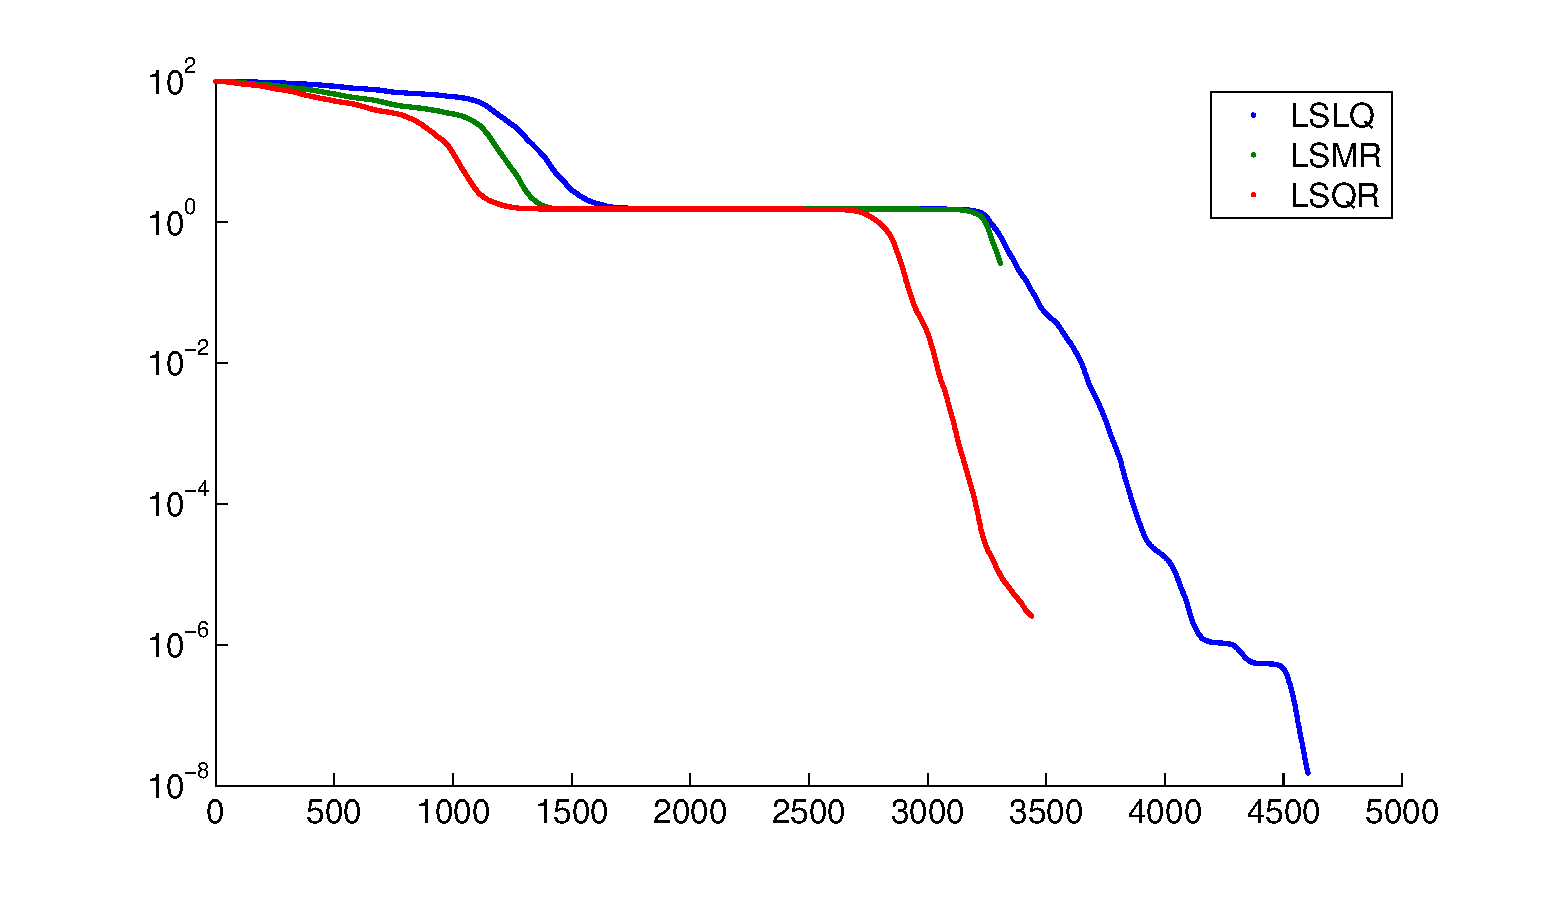
\includegraphics[width=0.48\textwidth]{Figures/Kemelmacher/forwarderror.eps}	
	}
	\hfill
	\subfigure[$\Vert A^T r_k \Vert_2$ per iteration]
	{
		\label{fig:kemel2}
		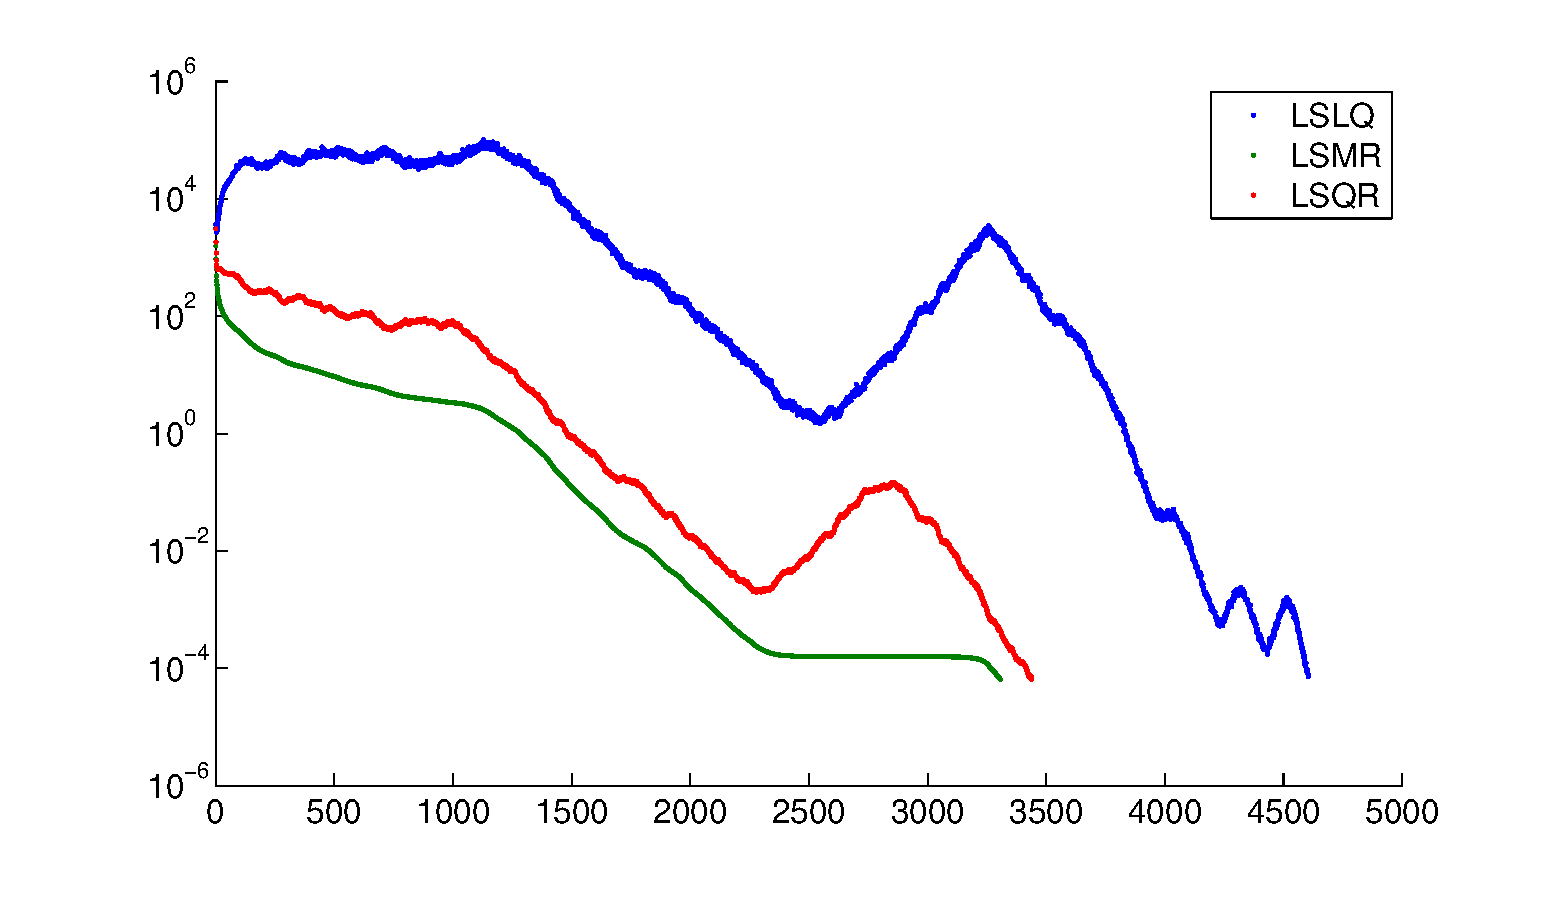
\includegraphics[width=0.48\textwidth]{Figures/Kemelmacher/normAr.eps}	
	}
	
	\subfigure[$\Vert r_k \Vert_2$ per iteration]
	{	
		\label{fig:kemel3}
		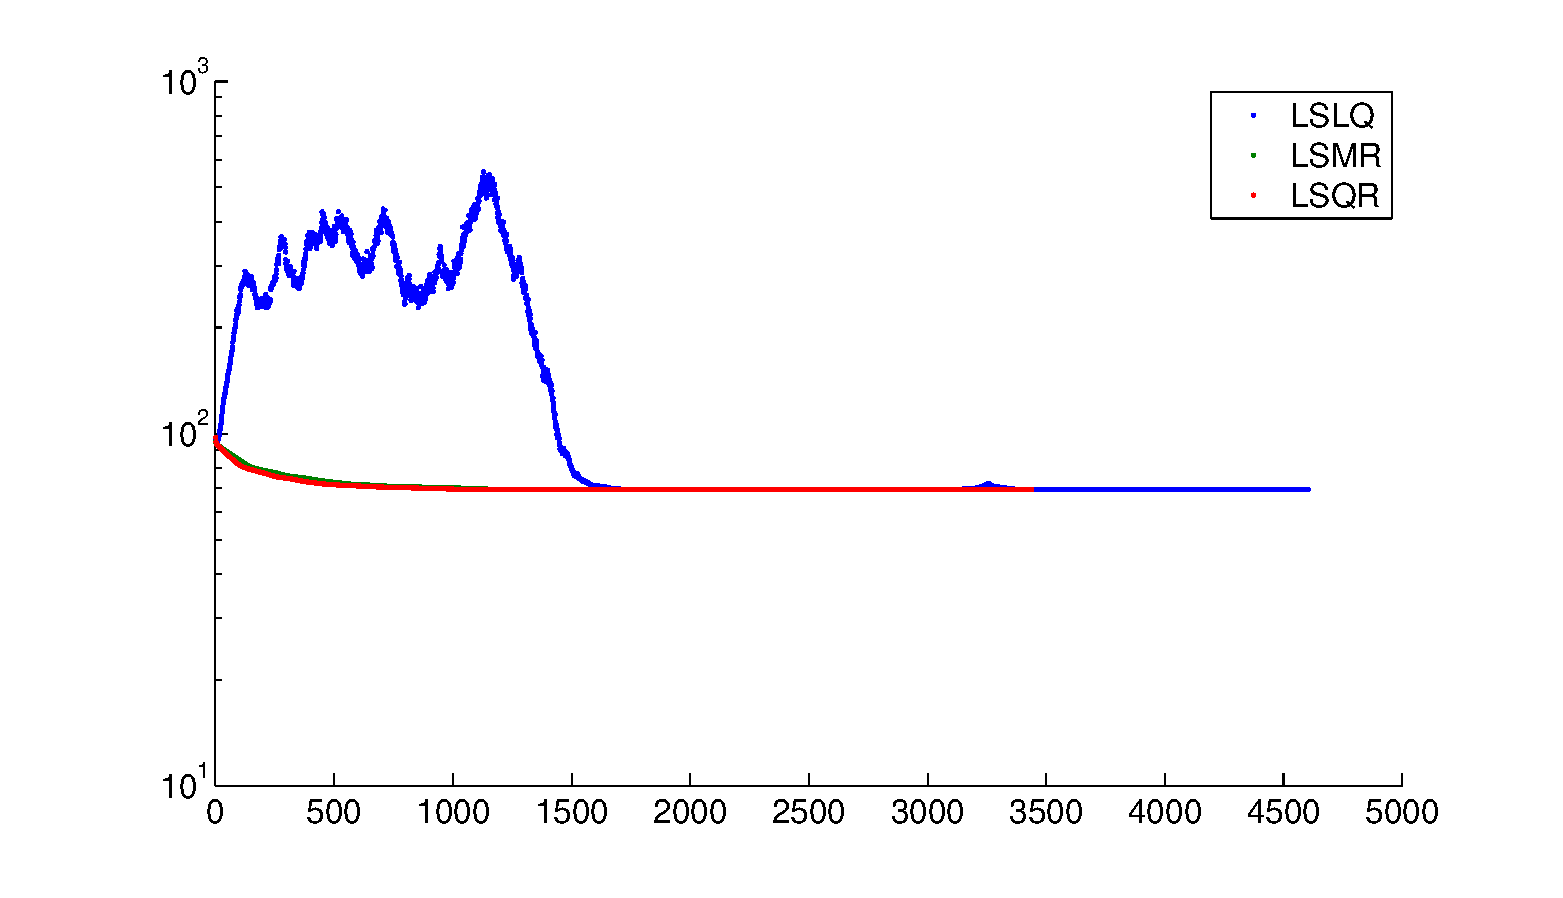
\includegraphics[width=0.48\textwidth]{Figures/Kemelmacher/normr.eps}	
	}
	\hfill
	\subfigure[$\Vert x_* - x_k \Vert_2$ vs. $\Vert A^T r_k \Vert_2$]
	{
		\label{fig:kemel4}
		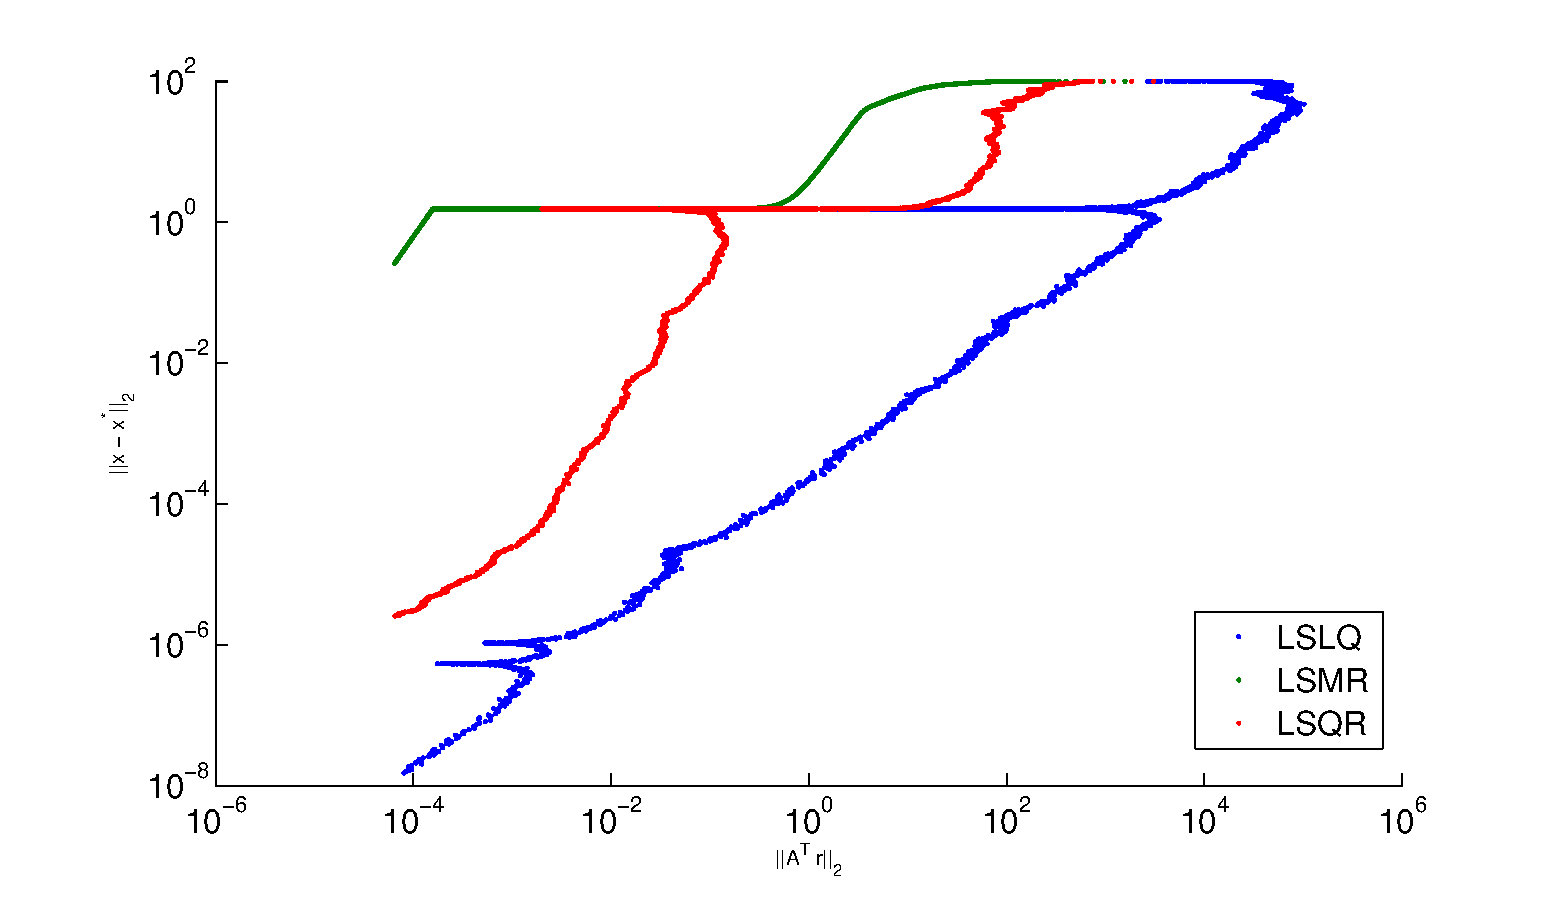
\includegraphics[width=0.48\textwidth]{Figures/Kemelmacher/forwarderrvsAr.eps}	
	}
	
	\caption{LSLQ, LSQR and LSMR results when run on the Kemelmacher problem.}
\end{figure}

It is evident that LSLQ lags behind both LSQR and LSMR for minimizing the forward error, $A^T r_k$ and the residual. Furthermore, LSQR and LSMR guarantee monotonic decrease in the residual $r_k$ (as CG and MINRES guarantee this for positive definite systems such as the normal equations), whereas LSLQ may increase the residual substantially as the iterations progress before converging towards a similar residual norm.

On the other hand, LSLQ demonstrates an interesting property that upon convergence according to the stopping criteria, it obtains a solution that is closer to the true solution by two orders of magnitude. Even though all 3 methods terminated according to the same stopping criteria, which is based on the residual, LSLQ produced the smallest error in the end. Although LSLQ was lagging behind LSMR and LSQR, it appears that upon termination LSLQ would be able to guarantee better bounds on the forward error, at the cost of more iterations. Remark that LSMR was the first to terminate due to it minimizing $\Vert A^T r_k \Vert_2$, but the solution it found had an error from the true solution orders of magnitude much larger than either LSQR or LSLQ.

This phenomenon is illustrated in Figure \ref{fig:kemel4}, where we plot $\Vert x_* - x_k \Vert_2$ on the vertical axis, and $\Vert A^T r_k \Vert_2$ on the horizontal axis. This plot should be read right to left, as initially $\Vert A^T r_k \Vert$ is large and is being decreased as the iterations progress. Let $x^{LQ}_\ell$, $x^{QR}_p$, and $x^{MR}_k$ be the iterates for LSLQ, LSQR, and LSMR at the $\ell$, $p$ and $k$ iterations respectively. This figure then shows that if
$$ \Vert A^T (b - A x^{LQ}_\ell) \Vert_2 \approx \Vert A^T (b - A x^{QR}_p) \Vert_2 \approx \Vert A^T (b - A x^{MR}_k) \Vert_2,$$
then
$$ \Vert x_* - x^{LQ}_\ell \Vert_2 \leq \Vert x_* - x^{QR}_p \Vert_2 \leq \Vert x_* -  x^{MR}_k \Vert_2.$$
It may be possible to estimate $\Vert x_* - x_k \Vert_2$ in SYMMLQ, and if a reasonable upper bound can be established per iteration, then transferring to the CG as in SYMMLQ would produce a method which would take roughly as many iterations as LSQR while guaranteeing sharper bounds on the forward error.

We repeat this experiment for lp\_osa\_30, which is a least squares problem of size $104374 \times 4350$ obtained from the Tim Davis Sparse matrix collection. We present the results in Figures \ref{fig:lp301}-\ref{fig:lp304}.

\begin{figure}[ht]
\centering
	\subfigure[$\Vert x_* - x_k \Vert_2$ per iteration]
	{
		\label{fig:lp301}
		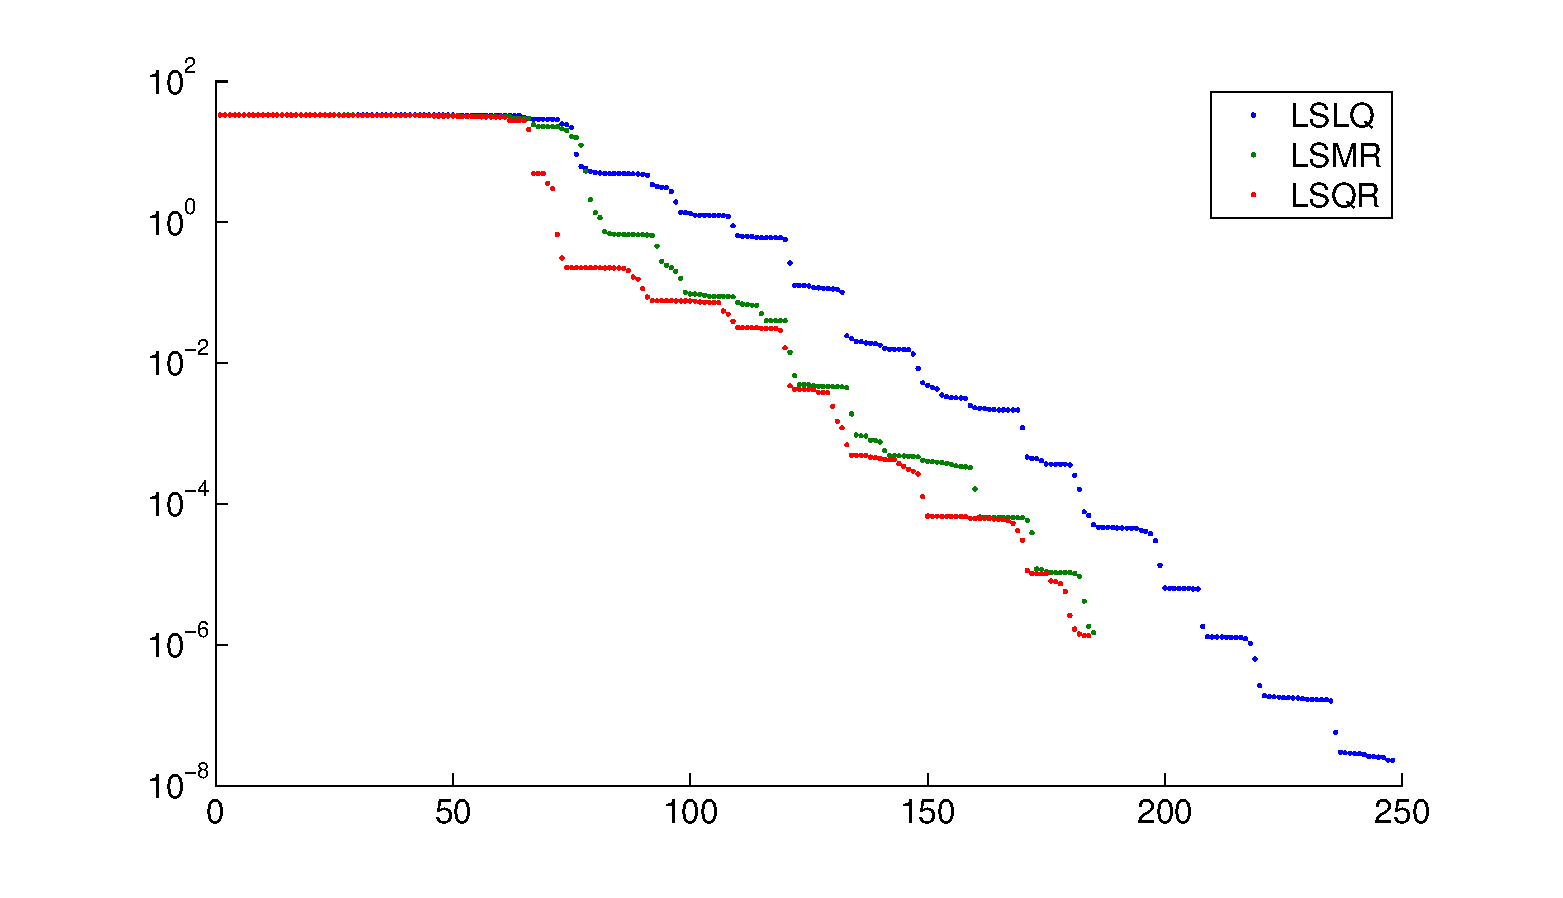
\includegraphics[width=0.48\textwidth]{Figures/lposa30/forwarderror.eps}	
	}
	\hfill
	\subfigure[$\Vert A^T r_k \Vert_2$ per iteration]
	{
		\label{fig:lp302}
		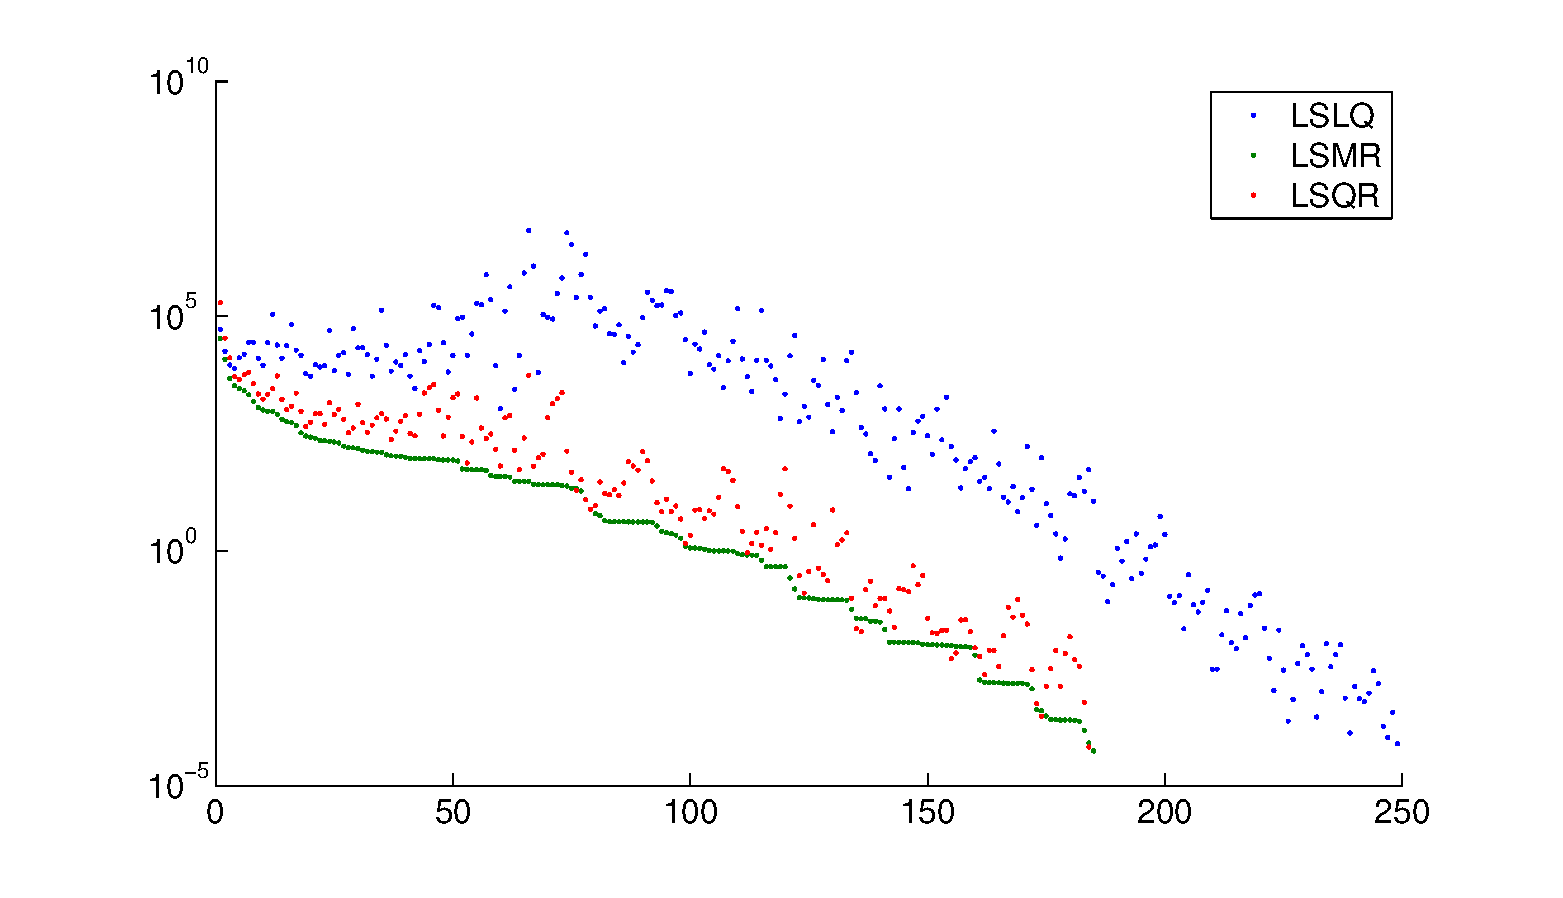
\includegraphics[width=0.48\textwidth]{Figures/lposa30/normAr.eps}	
	}
	
	\subfigure[$\Vert r_k \Vert_2$ per iteration]
	{	
		\label{fig:lp303}
		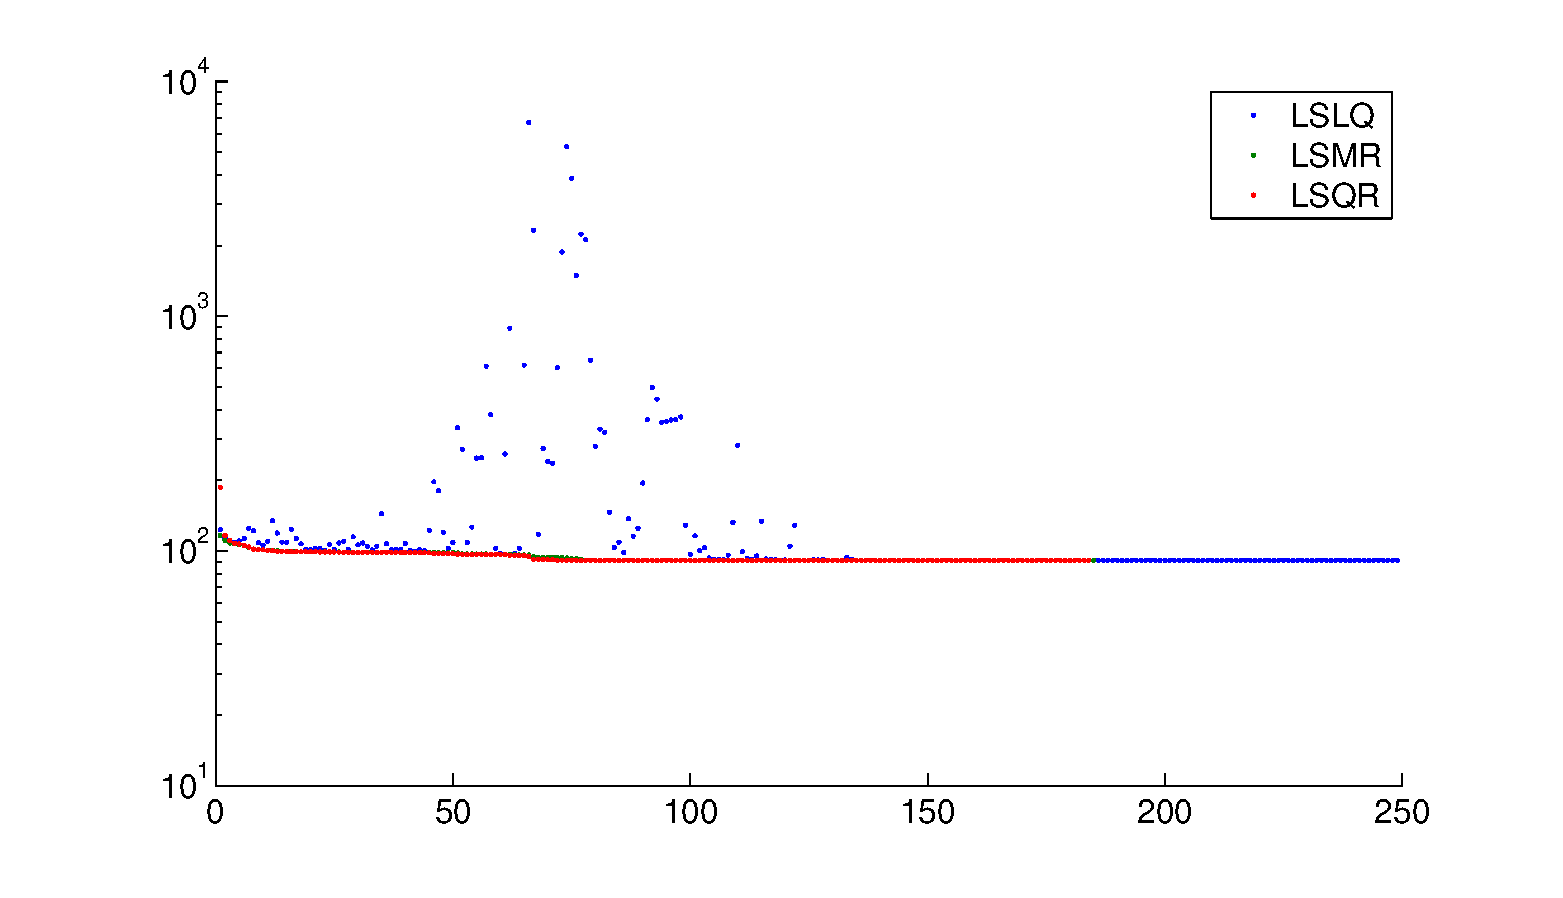
\includegraphics[width=0.48\textwidth]{Figures/lposa30/normr.eps}	
	}
	\hfill
	\subfigure[$\Vert x_* - x_k \Vert_2$ vs. $\Vert A^T r_k \Vert_2$]
	{
		\label{fig:lp304}
		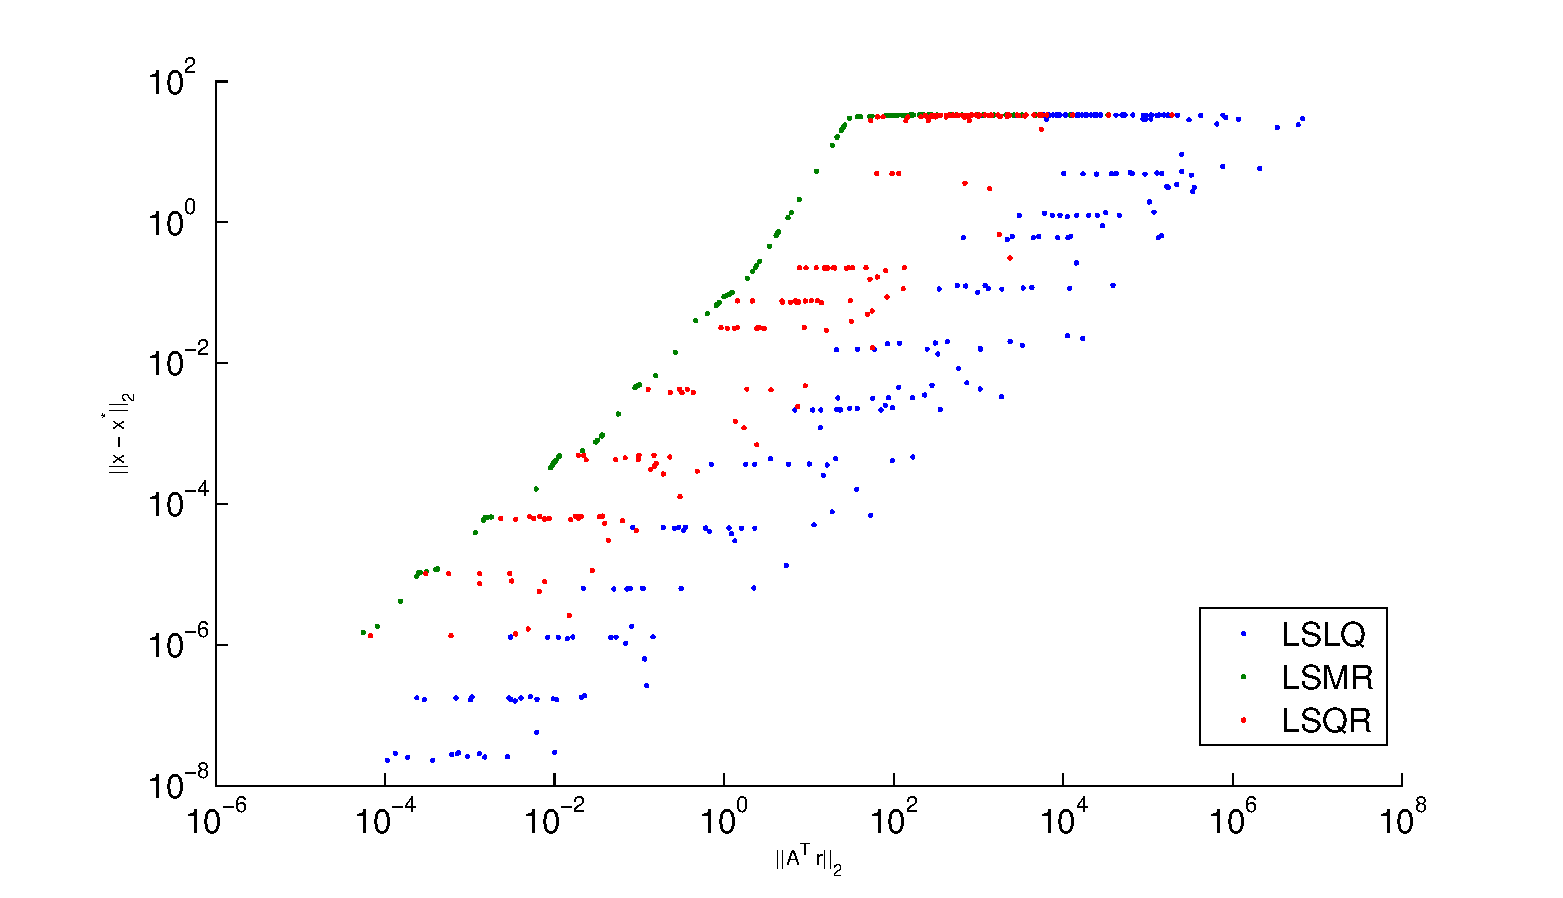
\includegraphics[width=0.48\textwidth]{Figures/lposa30/forwarderrvsAr.eps}	
	}
	
	\caption{LSLQ, LSQR and LSMR results when run on the lpo\_sa\_30 problem.}
\end{figure}

The results in this case are very similar to what was seen when the three methods were applied to the Kemelmacher problem.

We now test LSLQ on a nonsymmetric nonsingular square matrix. We take rdb3200l from the Tim Davis Sparse matrix collection, which is a $3200 \times 3200$ matrix. We plot the results in Figures \ref{fig:rdb1}-\ref{fig:rdb5}. These figures plot the same things as in the least squares problems, but we add figure \ref{fig:rdb5}, which plots $\Vert x_* - x_k \Vert_2$ against $\Vert r_k \Vert$, since we expect $r_k \rightarrow 0$ since the system is nonsingular. Note that since the problem is nonsingular now, the termination criteria is based on $\Vert r_k \Vert_2 \leq 10^{-10} \Vert b \Vert$.

\begin{figure}[ht]
\centering
	\subfigure[$\Vert x_* - x_k \Vert_2$ per iteration]
	{
		\label{fig:rdb1}
		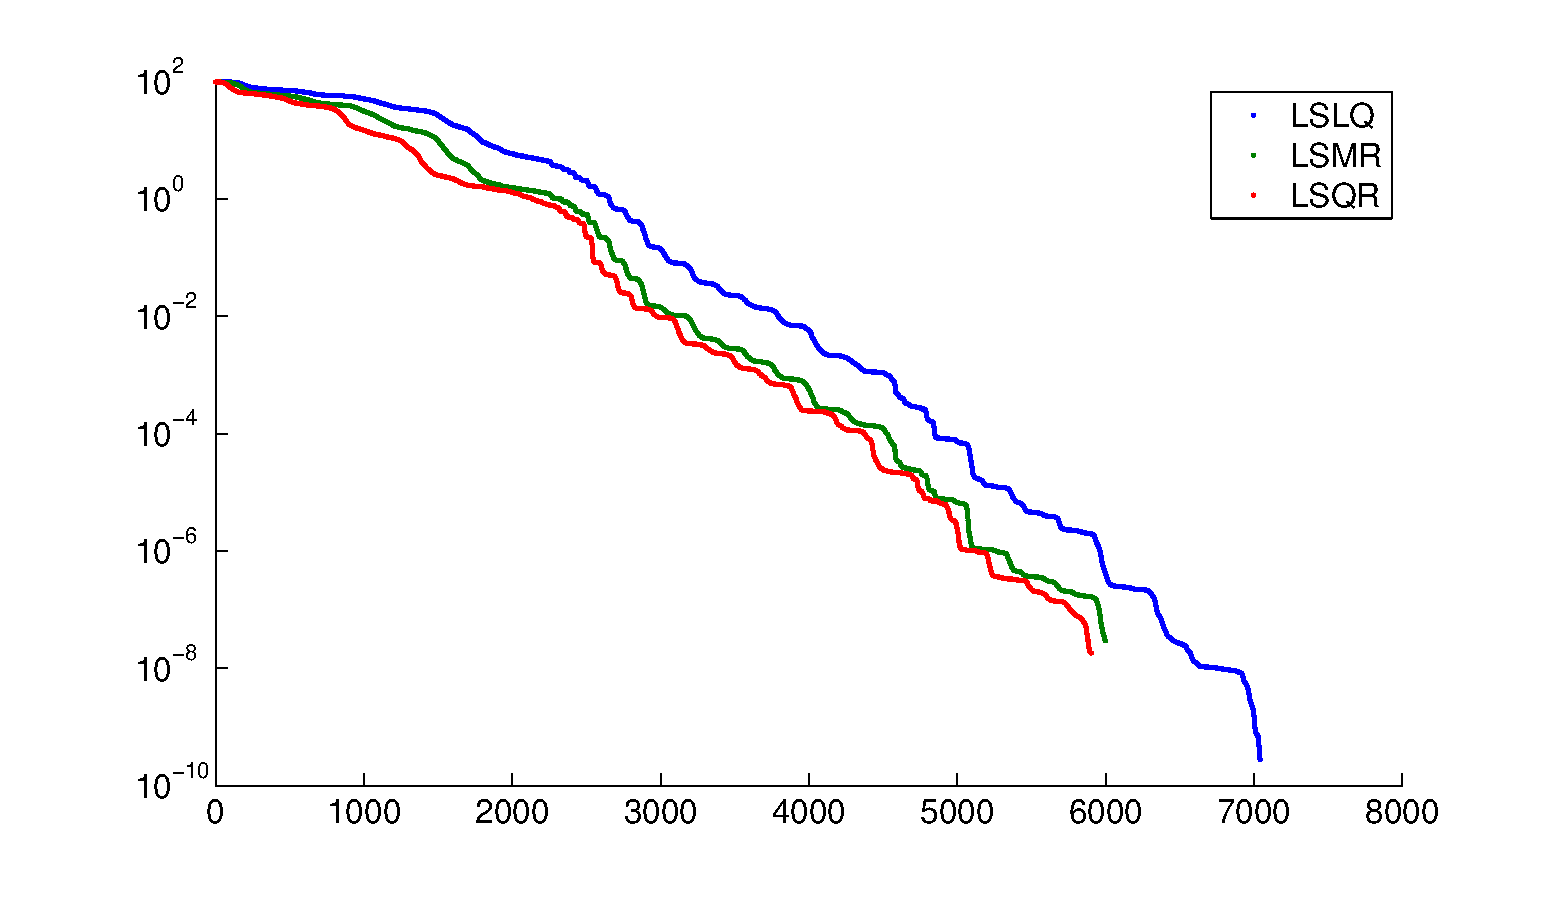
\includegraphics[width=0.48\textwidth]{Figures/rdb3200l/forwarderror.eps}	
	}
	\hfill
	\subfigure[$\Vert A^T r_k \Vert_2$ per iteration]
	{
		\label{fig:rdb2}
		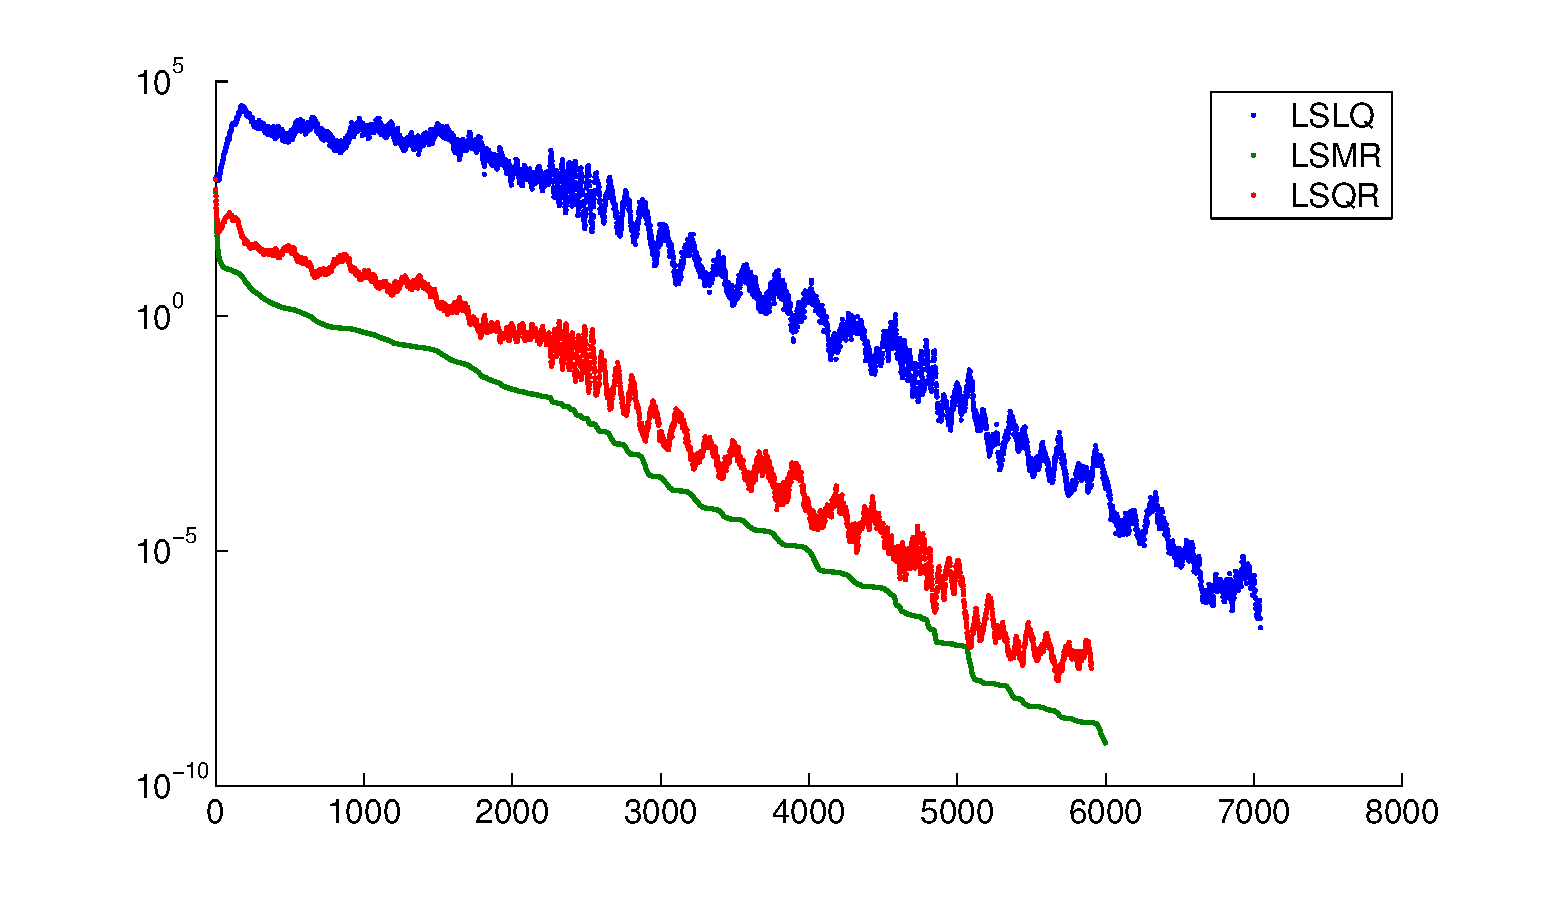
\includegraphics[width=0.48\textwidth]{Figures/rdb3200l/normAr.eps}	
	}
	
	\subfigure[$\Vert r_k \Vert_2$ per iteration]
	{	
		\label{fig:rdb3}
		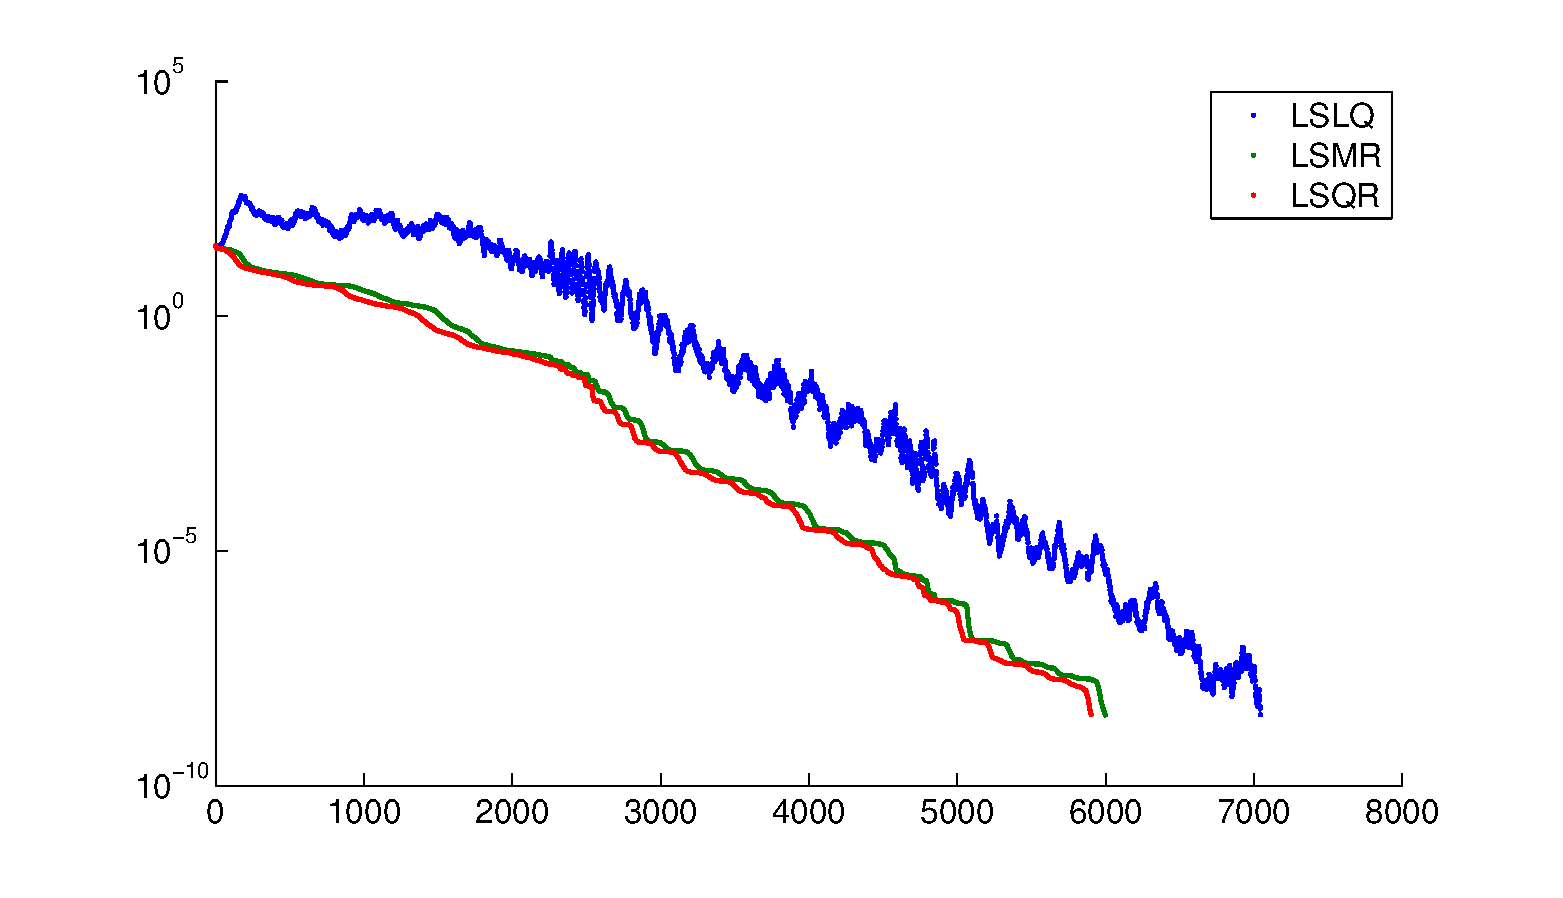
\includegraphics[width=0.48\textwidth]{Figures/rdb3200l/normr.eps}	
	}
	\hfill
	\subfigure[$\Vert x_* - x_k \Vert_2$ vs. $\Vert A^T r_k \Vert_2$]
	{
		\label{fig:rdb4}
		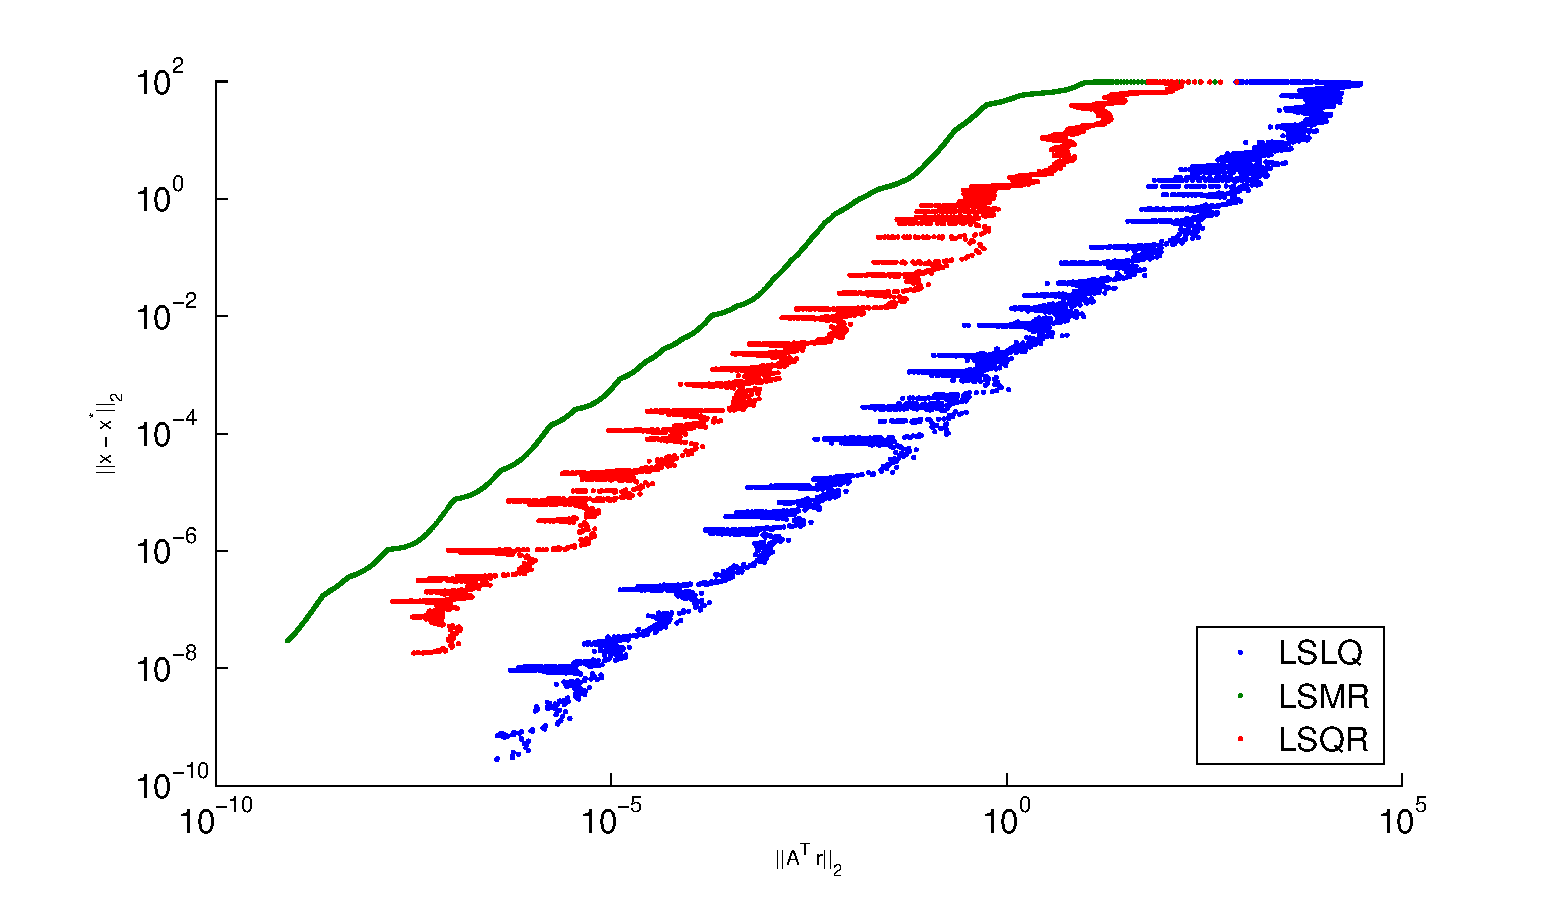
\includegraphics[width=0.48\textwidth]{Figures/rdb3200l/forwarderrvsAr.eps}	
	}
	
	\subfigure[$\Vert x_* - x_k \Vert_2$ vs. $\Vert r_k \Vert_2$]
	{
		\label{fig:rdb5}
		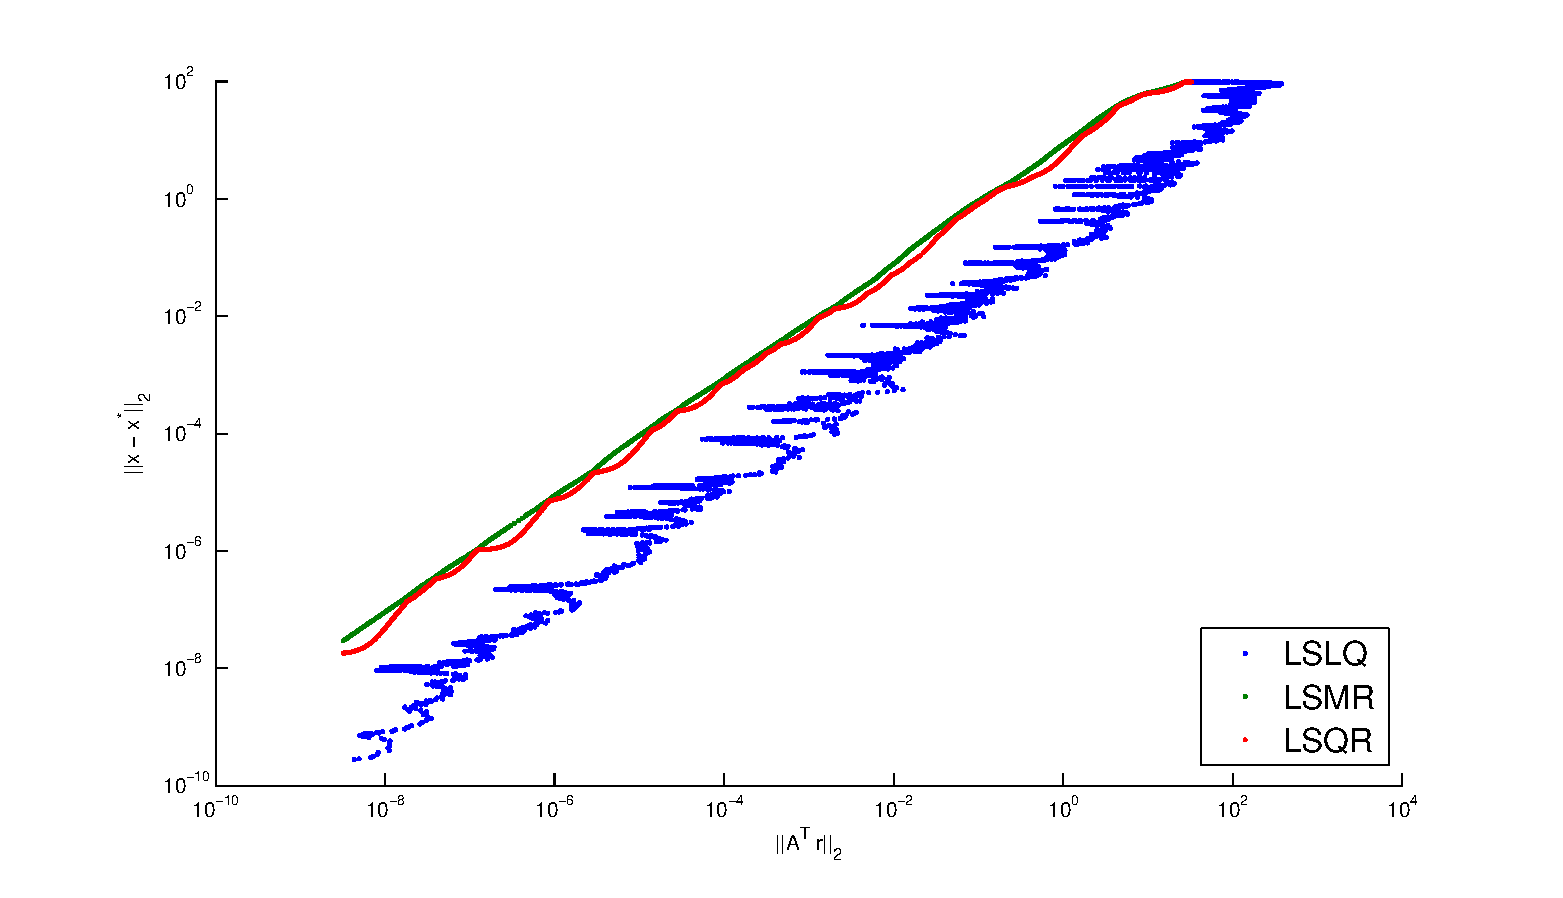
\includegraphics[width=0.48\textwidth]{Figures/rdb3200l/forwarderrvsr.eps}	
	}	
	
	\caption{LSLQ, LSQR and LSMR results when run on the rdb3200l problem.}
\end{figure}

The behaviour on this problem for the three methods is qualitatively no different from what was seen in the least squares problem. LSLQ lags behind the other methods based on the norm of the residual, $A^T r_k$, and the forward error. Interestingly, we do see LSQR perform slightly better than LSMR based on the residual, while LSMR consistently maintains a lower $\Vert A^T r_k \Vert_2$ (as it should be minimizing it for every iteration). But upon termination, LSLQ achieves a forward error 2 orders of magnitude lower than LSQR and LSMR, even though they all terminate around the same value of $\Vert r_k \Vert_2$. This phenomenon is again captured in figures \ref{fig:rdb4} and \ref{fig:rdb5}, where for similar residuals, LSLQ attains a lower forward error.

\section{Conclusion}
LSLQ is a method equivalent to SYMMLQ being applied to the normal equations has been derived and implemented in this project, in an approach similar to LSMR and LSQR. We've applied the method to several problems to investigate the performance of LSLQ compared to LSMR and LSQR, and found that although it does not converge as quickly as LSMR and LSQR to the solution, upon termination it appears to guarantee a lower forward error, often by over one order of magnitude, at the cost of more iterations. If an upper bound can be developed for $\Vert x_* - x_k \Vert_2$ to monitor the progress of LSLQ, and coupled with an upper bound on the error after transferring to the CG point, LSLQ can be a method that has performance similar to LSQR with stronger guarantees.

\end{document}